\documentclass[11pt]{article}
\usepackage{icmlko}
\begin{document}

\title{제 것이 아니었다 --- 팝업이 원핫에서 번 것은 남의 원핫이 꺼졌기 때문이다}
\author{월드모델 실험실}
\date{노트 403 · 2026년 8월 1일}
\maketitle

\begin{abstract}
노트 400과 402가 팝업(학습 24행)에 대해 정반대로 보였다 --- 드롭아웃
(원핫을 행마다 무작위로 끔)엔 $+0.0276 \cdot 12/12$ 로 \textbf{벌고},
학습 문턱 40(24행을 학습에서 통째로 뺌)엔 $-0.0525 \cdot 1/12$ 로
\textbf{잃는다}. 읽기는 깔끔했다: \emph{팝업은 제 행을 원하고 제 원핫을
원치 않는다.} 24행은 공유 축 모형에 보탬이 될 만큼은 되지만 제 원핫 열
하나를 세울 만큼은 안 된다.

처방을 사전 등록하고 관문에 올렸다 --- \textbf{원핫을 크기로 거른다}:
학습 행 40 이상인 도메인만 원핫 열을 갖고, 팝업은 \textbf{행은 그대로
학습에 넣되} 원핫만 전부 0. 예측 때 안 본 도메인이 받는 좌표와 같은 좌표다.

\begin{center}
\begin{tabular}{lrrr}
\hline
팝업에 한 일 & 팝업 변화 & 부호 \\
\hline
드롭아웃 $p{=}0.5$ (\textbf{전 도메인} 원핫을 끔) & $+0.0276$ & $12/12$ \\
\textbf{크기 원핫} (\textbf{팝업 원핫만} 없앰) & $\mathbf{+0.0006}$ & $8/12$ \\
문턱 40 (팝업 \textbf{24행}을 학습에서 뺌) & $-0.0525$ & $1/12$ \\
\hline
\end{tabular}
\end{center}

\textbf{50분의 1이다.} 판도 $+0.0002 \cdot 8/12$ 로 아무 일도 안 일어났다.
사전 등록에 적어 둔 실패 조건이 그대로 걸렸다 --- \emph{팝업이 안 벌면
노트 400의 $+0.0276$ 은 드롭아웃이 남의 원핫도 껐기 때문이지 제 원핫 탓이
아니었다는 뜻이다.} \textbf{이 갈래는 닫힌다.}
\end{abstract}

\section{읽기를 어디서 틀렸나}

``팝업은 제 원핫을 원치 않는다''는 드롭아웃 실험에서 팝업만 떼어 읽은
것이었다. 드롭아웃은 \textbf{열한 도메인의 원핫을 전부} 행마다 껐다.
팝업이 번 $+0.0276$ 은 제 원핫이 꺼져서가 아니라 \textbf{남들의 원핫이
꺼져서}였다 --- 모형이 도메인 이름표에 기댈 수 없게 되면 공유 축을 더 잘
쓰게 되고, 자기 이름표가 24행짜리라 애초에 쓸모없던 팝업이 그 개선을
고스란히 받는다. \textbf{팝업은 공유 축에 얹혀 가는 도메인이다.}

거꾸로 문턱 40의 $-0.0525$ 는 그대로 남는다. 그것은 원핫 이야기가 아니라
\textbf{24행이 축 모형에서 빠지는} 이야기이고, 노트 402가 잰 것이 맞다.

\section{왜 이렇게까지 작은가}

팝업의 원핫은 F18 학습 행 약 19{,}000 개 중 \textbf{24 개}에서만 1 이다
(0.13\%). 그 열 하나를 지우면 나무가 볼 것이 사실상 안 바뀐다. 열한 도메인
중 아홉이 $+0.0000 \sim +0.0008$ 사이에 $8/12$ 로 몰려 있는 것도 같은 이야기다
--- 쓸모없는 열 하나를 뺀 만큼 아주 조금씩 나아지지만 크기가 씨앗 잡음
($\pm 0.0033$, 노트 395)의 \textbf{16분의 1}이다.

규약대로면 판 $+0.0002 \cdot 8/12$ 는 조건 ①·② 를 다 못 넘어 36뽑기로
가야 한다. \textbf{안 돌렸다} --- 36뽑기가 어느 쪽으로 갈라지든 채택 후보는
사전 등록이 요구한 $+0.03$ 의 50분의 1이라 처방이 죽은 것은 이미 정해졌고,
규약의 마지막 항도 미결정이면 \textbf{유지}다. 결론이 안 바뀌는 계산은
안 한다.

\section{남은 것}

\begin{tabular}{lp{7.4cm}}
\hline
공유 축에 얹혀 가는 도메인 & 남의 원핫을 끄면 팝업이 번다 --- 원핫이 큰
도메인의 성적을 어떻게 사는지 되짚을 실마리. 노트 401이 못 찾은 값의 출처
쪽이다 \\
팝업 표본 & 내부 팝업 레코드는 통틀어 99건(2024:25 · 2025:50 · 2026:24)이고
그 중 89건이 판에 든다. \textbf{열 건이 어디서 빠지는지} 아직 안 봤다 \\
세 번째 전이 짝 & CN 만화 2025+ 19행 \\
\hline
\end{tabular}

\begin{figure}[h]
\centering
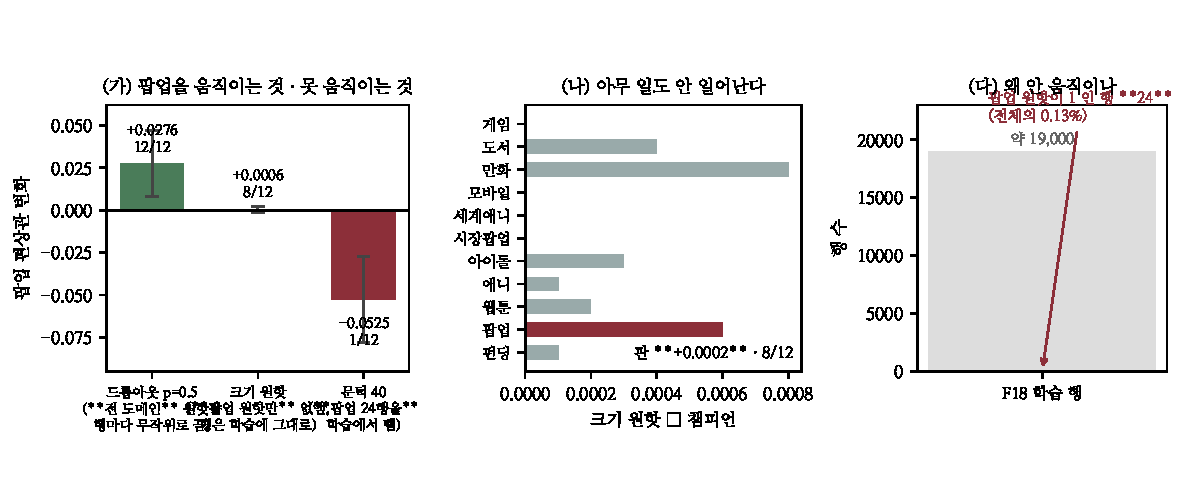
\includegraphics[width=\textwidth]{figs/fig403.pdf}
\caption{(가) 팝업을 움직이는 조작과 못 움직이는 조작. 제 원핫만 없애는
것은 아무것도 안 한다. (나) 열한 도메인 전부 $|{\cdot}| \le 0.0008$.
(다) 팝업 원핫이 1 인 학습 행은 24 --- 전체의 0.13\%.}
\end{figure}

\end{document}
